\documentclass[a4paper,11pt]{article}

\usepackage{titlesec}

\setcounter{secnumdepth}{4}

\titleformat{\paragraph}
{\normalfont\normalsize\bfseries}{\theparagraph}{1em}{}
\titlespacing*{\paragraph}
{0pt}{3.25ex plus 1ex minus .2ex}{1.5ex plus .2ex}

\usepackage[utf8]{inputenc}
\usepackage[T1]{fontenc} % LY1 also works
\usepackage[margin=1in]{geometry}

%% Font settings suggested by fbb documentation.
\usepackage{textcomp} % to get the right copyright, etc.
\usepackage[lining,tabular]{fbb} % so math uses tabular lining figures
\usepackage[scaled=.95,type1]{cabin} % sans serif in style of Gill Sans
\usepackage[varqu,varl]{zi4}% inconsolata typewriter
\useosf % change normal text to use proportional oldstyle figures
%\usetosf would provide tabular oldstyle figures in text

\usepackage{microtype}
\usepackage{siunitx}
\DeclareSIUnit{\belmilliwatt}{Bm}
\DeclareSIUnit{\dBm}{\deci\belmilliwatt}
\sisetup{range-phrase=--, range-units=single, binary-units = true}
\usepackage{graphicx}
\usepackage{tikz}
\usepackage{svg}
%\usepackage{hyperref}
\usetikzlibrary{arrows, shadows}
\tikzset{%
  cascaded/.style = {%
    general shadow = {%
      shadow scale = 1,
      shadow xshift = -1ex,
      shadow yshift = 1ex,
      draw,
      thick,
      fill = white},
    general shadow = {%
      shadow scale = 1,
      shadow xshift = -.5ex,
      shadow yshift = .5ex,
      draw,
      thick,
      fill = white},
    fill = white, 
    draw,
    thick,
    minimum width = 1.5cm,
    minimum height = 2cm}}
    
\usepackage{enumitem}
\setitemize{noitemsep,topsep=0pt,parsep=0pt,partopsep=0pt}
\setenumerate{noitemsep,topsep=0pt,parsep=0pt,partopsep=0pt}
\setlist{leftmargin=*}
\usepackage{listings}
\lstset{
	basicstyle=\ttfamily,
	frame=single,
	breaklines=true,
	morecomment=[l][\color{green}]{\#},
}
\usepackage[os=win]{menukeys}
\renewmenumacro{\keys}[+]{shadowedroundedkeys}

\usepackage{booktabs,caption}
\usepackage[flushleft]{threeparttable}
\newcolumntype{L}[1]{>{\raggedright\let\newline\\\arraybackslash\hspace{0pt}}m{#1}}
\newcolumntype{C}[1]{>{\centering\let\newline\\\arraybackslash\hspace{0pt}}m{#1}}
\newcolumntype{R}[1]{>{\raggedleft\let\newline\\\arraybackslash\hspace{0pt}}m{#1}}
\usepackage{tabularx} 

\usepackage{multirow}

\usepackage{stackengine}
\usepackage{scalerel}
\usepackage{xcolor,mdframed}

\newcommand\danger[1][5ex]{%
  \renewcommand\stacktype{L}%
  \scaleto{\stackon[1.3pt]{\color{red}$\triangle$}{\tiny !}}{#1}%
}

\newenvironment{important}[1][]{%
   \begin{mdframed}[%
      backgroundcolor={red!15}, hidealllines=true,
      skipabove=0.7\baselineskip, skipbelow=0.7\baselineskip,
      splitbottomskip=2pt, splittopskip=4pt, #1]%
   \makebox[0pt]{% ignore the withd of !
      \smash{% ignor the height of !
         %\fontsize{32pt}{32pt}\selectfont% make the ! bigger
         \hspace*{-45pt}% move ! to the left
         \raisebox{-5pt}{% move ! up a little
            {\danger}% type the bold red !
         }%
      }%
   }%
}{\end{mdframed}}

\newcommand\info[1][5ex]{%
  \renewcommand\stacktype{L}%
  \scaleto{\stackon[1.2pt]{\color{blue}$\bigcirc$}{\raisebox{-1.5pt}{\small i}}}{#1}%
}

\newenvironment{information}[1][]{%
   \begin{mdframed}[%
      backgroundcolor={blue!15}, hidealllines=true,
      skipabove=0.7\baselineskip, skipbelow=0.7\baselineskip,
      splitbottomskip=2pt, splittopskip=4pt, #1]%
   \makebox[0pt]{% ignore the withd of !
      \smash{% ignor the height of !
         %\fontsize{32pt}{32pt}\selectfont% make the ! bigger
         \hspace*{-45pt}% move ! to the left
         \raisebox{-5pt}{% move ! up a little
            {\info}% type the bold red !
         }%
      }%
   }%
}{\end{mdframed}}

\usepackage{makecell}
\usepackage{hyperref}
\newcommand{\vna}{LibreVNA}

\newcommand{\screenshot}[2]{\begin{center}
\includegraphics[width=#1\textwidth]{Screenshots/#2}
\end{center}}

\title{\vna{} User Manual}
%\author{Jan Käberich (\url{j.kaeberich@gmx.de})}
\begin{document}
\maketitle

%\begin{abstract}
%The Testcard is a platform for the characterization of small energy sources. It is able to charge/discharge up to eight energy sources with a predefined pattern and record their voltages.
%\end{abstract}

\setcounter{tocdepth}{3}
\tableofcontents
\clearpage

%\section*{Nomenclature}
%
%\begin{description}
%\item[Testcard] Board with the hardware to characterize up to eight energy sources.
%\item[CLI] Command Line Interface. Program running on the computer which controls the testcard.
%\item[Channel] One of the eight measurement units on the testcard.
%\begin{description}
%\item[Voltage] Voltage of the energy source connected to the channel.
%\item[Current] Current flowing through the energy source connected to the channel. Defined as the current flowing from the energy source to the testcard, thus the source is discharged for positive and charged for negative values.
%\end{description}
%\item[Load] Application of a current at the channels for a specified timespan.
%\item[Measurement] Single measurement of channel voltages at a specified point in time.
%\item[Trace] Periodic measurement of channel voltages.
%\item[Sequence] A combination of loads, measurements and traces.
%\end{description}

\section{Overview}

\begin{tikzpicture}
\begin{scope}[xshift=1.5cm]
    \node[anchor=south west,inner sep=0] (image) at (0,0) {\includegraphics[width=0.76\textwidth]{TopDrawing.pdf}};
    \begin{scope}[x={(image.south east)},y={(image.north west)}]
		\node [anchor=south, align=center] (port1) at (0,1) {Port 1};
		\node [anchor=south, align=center] (port2) at (0,0.2) {Port 2};
		\node [anchor=west, align=center] (leds) at (1.05,0.8) {LEDs\\ \footnotesize Ready\\ \footnotesize Debug\\ \footnotesize Port1\\ \footnotesize Port2\\ \footnotesize Ext. Reference\\ \footnotesize Source unlocked\\ \footnotesize LO unlocked\\ \footnotesize FPGA unlocked\\ \footnotesize Booting\\ \footnotesize Power};
		\node [anchor=west, align=center] (power) at (1.05,0.5) {External Power \\ \footnotesize (optional)};
		\node [anchor=west, align=center] (usb) at (1.1,0.4) {USB};
		\node [anchor=west, align=center] (refout) at (1.1,0.2) {Reference\\Output};
		\node [anchor=west, align=center] (refin) at (1.1,0) {Reference \\Input};

        \draw [-*, ultra thick, gray] (port1) to[] (0.02,0.89);
        \draw [-*, ultra thick, gray] (port2) to[] (0.02,0.09);
        \draw [-*, ultra thick, gray] (leds) to[] (0.8,0.84);
        \draw [-*, ultra thick, gray] (power) to[] (0.91,0.55);
        \draw [-*, ultra thick, gray] (usb) to[] (0.91,0.5);
        \draw [-*, ultra thick, gray] (refout) to[] (0.97,0.23);
        \draw [-*, ultra thick, gray] (refin) to[] (0.97,0.1);
    \end{scope}
\end{scope}
\end{tikzpicture}%

\subsection{USB}
The \vna{} uses a USB-C connector as the power supply and for data transmission. The hardware supports the USB power delivery standard\footnote{Work in progress, the device will not negotiate USB-PD yet}, requires \SI{5}{\volt} and draws up to \SI{1.2}{\ampere} of current.

The implemented USB device is limited to USB 2.0 Fullspeed and data transmission will work with any USB 2.0 or 3.0 port (no USB-C required). However, the current consumption exceeds the specifications for USB 2.0 and 3.0 ports and the \vna{} may be unable to fully boot when no external power is applied and the USB host limits the current.
\subsection{External Power}
Input jack for external DC power (\SI{5}{\volt}, \SI{1.5}{\ampere}, positive center pin). If a power source is connected, no current is drawn from the USB port anymore.
\subsection{RF ports}
RF connector to connect the DUT. Both ports are identical and the device architecture supports full S-Parameter measurements (S11, S21, S12 and S22).
\begin{important}
The RF ports have no input protection, so do not apply a signal with more than +\SI{10}{\dBm} of power.
\end{important}
\subsection{LEDs}
Ten LEDs indicate the status:
\begin{description}
\item [Ready (green)] Indicates fully booted \vna{}, ready to take measurements
\item [Debug (green)] Not used at the moment
\item [Port 1 (green)] Active output signal on port 1
\item [Port 2 (green)] Active output signal on port 2
\item [Ext. Reference (green)] External reference in use
\item [Source unlocked (red)] The source PLL failed to lock (it may turn on briefly during a sweep, this is not a problem)
\item [LO unlocked (red)] The 1.LO PLL failed to lock (it may turn on briefly during a sweep, this is not a problem)
\item [FPGA unlocked (red)] The FPGA clock PLL failed to lock
\item [Booting (red)] Indicates boot process, also used for error codes
\item [Power (green)] USB power valid
\end{description}
\subsection{Reference Output}
Optional reference output port (user selectable \SI{10}{\mega\hertz} or \SI{100}{\mega\hertz}). The output power is approximately +\SI{3}{\dBm}.
\subsection{Reference Input}
High impedance reference input port. When applying a \SI{10}{\mega\hertz} input signal, it can be used to overwrite the internal TCXO.
\begin{information}
Due to the high impedance input, the external input may detect a valid signal when picking up external radiation. If this is a problem, either terminate the reference input connector or disable automatic reference switching.
\end{information}

\section{Getting started}
\begin{enumerate}
\item Connect the \vna{} to a computer using the USB port. After a couple of seconds, only the "Power" and "Ready" LEDs should stay on. If the "Ready" LED does not turn on or the "Booting" LED indicates an error code, there is a problem and the device will not function properly. See section~\ref{troubleshooting} for possible solutions.
\item Start the PC application to connect to the \vna{}. The window should look similar to this:
\makebox[\textwidth][c]{
\includegraphics[width=\textwidth]{Screenshots/ApplicationOverview.png}
}
\end{enumerate}
\subsection{GUI element types}
The \vna{} application is made up of six areas containing different types of control:
\begin{itemize}
\item The \textbf{Trace Display Area} shows the measured data in various diagrams.
\item The \textbf{Toolbars} provide access to commonly used device settings. They can be rearranged or disabled (see section~\ref{menu:window}).
\item The \textbf{Menu} at the top left handles less common settings or more complex actions (often with additional popup windows).
\item The \textbf{Docks} mostly provide access to display related settings such as traces and markers. They can be rearranged or disabled (see section~\ref{menu:window}).
\item The \textbf{Statusbar} at the bottom show some basic informations about the connected device. If error conditions (e.g. ADC overload) are present, they are indicated at the bottom right corner.
\item The \textbf{Modeswitch} at the top right allows changing the \vna{} operating mode. Although it is primarily designed as a vector network analyzer, the hardware architecture allow some other operating modes with certain limitations.
\end{itemize}
Depending on the current operating mode, the available toolbars, docks and menu entries change. It is also possible to rearrange the docks and toolbars.

\subsection{Common GUI elements}
Certain control elements are always available, regardless of the selected mode. They control settings of the \vna{} that are not specific to any of the operating modes.

\paragraph{Entering values}\hfill\newline
Most entry fields support SI prefixes. To set a new value, type in the number followed by an SI prefix (e.g. to set \SI{3.2}{\giga\hertz} press \keys{3},\keys{.},\keys{2},\keys{\shift+G}). The accepted prefixes vary depending on the input (e.g. pico is a valid prefix for a capacitance while it will not be accepted for a frequency). 

\subsubsection{Reference Toolbar}
The reference toolbar controls the external reference output as well as the input.
\screenshot{0.5}{ToolbarReference.png}
The reference can be set to "Int" (internal TCXO), "Ext" (external \SI{10}{\mega\hertz} signal) or to automatic mode. In automatic mode, the reference will switch to the external input when a signal is detected, otherwise it will use the internal TCXO.

The external reference output may either be disabled or set to \SI{10}{\mega\hertz} or \SI{100}{\mega\hertz}.

\subsubsection{Device Log Dock}
This dock shows the debug output of the \vna{} (the same messages as on the internal UART port). It may help to identify problems, otherwise it is not required for operation.
\screenshot{1.0}{DockDeviceLog.png}

\subsubsection{File Menu}
Changing the default setup of the application can require a lot of configuration, especially if some of the more complicated math or de-embedding options are used. To simplify this process, setup-files can be saved and opened, which perform these steps automatically. A setup file contains all settings and configuration of these elements:
\begin{itemize}
\item Sweep and Acquisition settings (start/stop frequency, IF bandwidth, ...)
\item The currently active mode (VNA, Signalgenerator or Spectrumanalyzer)
\item Traces (Name, Color, Parameters, ...)
\item Math operations applied to the traces
\item Markers
\item De-embedding options
\item Graph setup and enabled traces
\end{itemize}
\begin{important}
If any part of the setup references another file (i.e. a trace imported from a touchstone file), only the filename is saved. Opening a setup file after moving/deleting any of the referenced files will result in missing data. 
\end{important}

\subsubsection{Device Menu}
The device menu controls the connection state, allows low level hardware access and to perform firmware updates:
\begin{itemize}
\item \textbf{Update Device List:} Scans the USB port for connected devices. Clicking this action simply updates the list of devices, no connection is established.
\item \textbf{Connect to:} Select which \vna{} to connect to. Different devices are identified by their serial number.
\item \textbf{Disconnect:} Disconnect from the \vna{}.
\item \textbf{Manual Control:} Starts the manual control dialog in which all hardware settings are accessible (mostly used for testing purposes):
\screenshot{1.0}{DialogManualControl.png}
\item \textbf{Firmware Update:} Load a new microcontroller firmware and FPGA configuration into the \vna{}. Do not disconnect power while updating the firmware!
\screenshot{0.6}{DialogFirmwareUpdate.png}
\end{itemize}

\subsubsection{Window Menu}
\label{menu:window}
The window menu allows hiding not needed toolbars and docks. It also contains some application preferences.

\section{Vector Network Analyzer}
In this operating mode, the \vna{} takes S-parameter measurements. A source signal is generated and alternately applied to the RF ports. The incoming signal at both RF ports is measured, resulting in the four S-parameters S11 and S21 (when the source signal is routed to port 1) as well as S12 and S22 (when it is routed to port 2).

\subsection{Signal processing architecture}
\label{vna:dsp}
This section contains some details of the signal flow inside the \vna{}-Application. Knowledge of the signal flow is not required to operate the \vna{} but may help to understand certain features and limitations.
\tikzstyle{block} = [draw, rectangle, 
    minimum height=3em, minimum width=6em]
\tikzstyle{sum} = [draw, fill=blue!20, circle, node distance=1cm]
\tikzstyle{input} = [coordinate]
\tikzstyle{output} = [coordinate]
\tikzstyle{pinstyle} = [pin edge={to-,thin,black}]
\tikzset{%
  cascaded/.style = {%
    general shadow = {%
      shadow scale = 1,
      shadow xshift = -1ex,
      shadow yshift = 1ex,
      draw,
      %thick,
      fill = white,
      },
    general shadow = {%
      shadow scale = 1,
      shadow xshift = -.5ex,
      shadow yshift = .5ex,
      draw,
      %thick,
      fill = white,
      },
    fill = white, 
    draw,
    %thick,
    %minimum width = 1.5cm,
    %minimum height = 2.1cm
    }}

% The block diagram code is probably more verbose than necessary
\begin{center}
\begin{tikzpicture}[auto, node distance=2cm,>=latex']
    % We start by placing the blocks
	\node [block] (VNA) {VNA Hardware};
	\node [block, below of=VNA] (cal) {Calibration};
	\node [block, below of=cal] (deemb)  {De-embedding};
	\node [cascaded, block, below of=deemb, align=center, node distance=3cm, minimum height=2cm] (traces)  {Traces\\ \\ \\};
	\node [block, dashed, minimum width=4em, minimum height=2em, below of=traces, node distance=0.2cm] (math) {Math};
	\node [cascaded, block, node distance=3cm, below of=traces] (graphs)  {Graphs};


	\draw [->] (VNA) -- node {uncalibrated S parameter set (S11,S12,S21,S22) over USB} (cal);
	\draw [->] (cal) -- node {calibrated S parameter set (S11,S12,S21,S22)} (deemb);
	\draw [->] (deemb) -- node {individual S parameters} ([yshift=1ex]traces.north);
	\node [left of=traces, node distance=4cm](import){};
	\draw [->] (import) -- node {imported files} ([xshift=-1ex]traces.west);
	\node [right of=traces, node distance=6cm](export){};
	\draw [->] (traces.east) -- node {CSV/Touchstone export} (export);
	\draw [->] (traces) -- node {complex frequency/time domain data} ([yshift=1ex]graphs.north);
\end{tikzpicture}
\end{center}

The central element of the signal flow is the concept of \textbf{traces}. A trace is created from a single S parameter across frequency (either measured by the \vna{} or imported from an external file). Once the data is captured in a trace, optional math operations may be applied to it (e.g. performing a TDR to transform the data into the time domain) and the result of these operations are passed on to the graphs.

When capturing data from the \vna{}, additional operations take place before the data is fed to the traces. First, the \vna{} measures the four S parameters between its two ports. The raw measurements are transferred through USB. The first processing block is the calibration (see also section~\ref{vna:calibration}), followed by optional de-embedding procedures. After the de-embedding, the four S parameters are split into individual S parameters and the relevant traces are updated.

This concept has several consequences when using the \vna{}, some of which are:
\begin{itemize}
\item You can always take calibration measurements. No matter how the de-embedding or math operations in the traces are set up, they will never influence the calibration routine
\item A valid calibration is required before using de-embedding options (otherwise, most de-embedding options won't be able to work properly)
\item Applying a calibration or de-embedding to traces imported from files is not possible
\item Once the data arrives in the traces, the S parameters are no longer associated (e.g. there is no connection between S11 and S21 anymore. It is possible to "pause" the trace capturing S11 while S21 continues to get updated)
\end{itemize}

\subsection{Sweep Toolbar}
This toolbar sets the swept frequency range.
\screenshot{1.0}{ToolbarSweep.png}
The start/stop and center frequency as well as the span can be set directly.

Additionally, the sweep toolbar contains buttons for zooming in/out around the center frequency and a preset to set the sweep to the full frequency range.
\subsection{Acquisition Toolbar}
\screenshot{0.7}{ToolbarVNAAcquisition.png}
\begin{itemize}
\item \textbf{Level:} The amount of power used for stimulus generation. The dynamic range decreases when using smaller values. It is recommended to use the highest available settings when measuring passive networks. When measuring active devices (e.g. amplifiers), decrease the stimulus power in such a way that the input power into any port does not rise above \SI{-10}{\dBm} to stay within the linear range of the \vna.
\item \textbf{Points:} Amount of measurement points in one sweep. More points provide finer frequency resolution but also increase sweep time.
\item \textbf{IF BW:} Bandwidth of final IF measurement. Low bandwidths increase the sweep time but improve the noisefloor. At higher frequencies (roughly above \SI{3}{\giga\hertz}), the dynamic range is limited by the isolation between the ports and decreasing the IF bandwidth does not improve the noisefloor anymore.
\item \textbf{Averaging:} Moving average across multiple sweeps.
\end{itemize}

\subsection{Traces}
Adding/configuring traces is handled by the \textbf{Trace Dock} (by default on the left side): 
\screenshot{0.3}{TraceDock.png}
The list shows all available traces, by default the four S parameters S11, S12, S21 and S22. Different icons in front of the trace names indicate the state of the trace. Clicking on one of the icons toggles the state:
\begin{itemize}
\item \includesvg[height=8pt]{Screenshots/visible}/\includesvg[height=10pt]{Screenshots/invisible}: Enable/disable global visibility: Shows/hides the trace an all graphs it is enabled on.
\item \includesvg[height=8pt]{Screenshots/play}/\includesvg[height=8pt]{Screenshots/pause}: Play/pause. Only available when the trace is fed from live VNA data, not when it was created from a touchstone file. Pausing a trace freezes the current data, new measurements from the \vna{} will not update the trace.
\item \includesvg[height=8pt]{Screenshots/math_enabled}/\includesvg[height=10pt]{Screenshots/math_disabled}: Enable/disable math. Only available if at least one math operation is present.
\end{itemize}
\noindent
Creating a new trace or double clicking on an existing trace opens the "edit trace" window:
\screenshot{1.0}{TraceEdit.png}
On the left side, additional trace parameters can be changed, while the right side of the window handles math operations that will be applied to the trace data. The available trace parameters are:
\begin{itemize}
\item \textbf{Name}
\item \textbf{Color}
\item \textbf{Velocity factor} (only relevant when transforming into the time domain)
\item \textbf{Data source} (Live Capture/From File/From Math)
\end{itemize}

\subsubsection{Trace Data Sources}
Every trace can receive its data from one of three source:
\begin{itemize}
\item \textbf{Live Capture:} Sampled data from the LibreVNA are added to the trace in real time
\item \textbf{From File:} Import static data from an external touchstone or CSV file
\item \textbf{From Math:} Combine data from other traces with math operations to create a new trace
\end{itemize}

\paragraph{Live Capture}
\screenshot{0.5}{LiveCapture.png}
The trace is constantly updated by the data received from a connected and sweeping LibreVNA. The available Live Capture parameters are:
\begin{itemize}
\item \textbf{Type:} Live Captures can be 3 different types:
\begin{itemize}
\item \textbf{Overwrite:} The trace data is overwritten each sweep
\item \textbf{Max hold:} The trace data with the highest signal magnitude is persisted
\item \textbf{Min hold:} The trace data with the lowest signal magnitude is persisted
\end{itemize}
\item \textbf{Parameter:} The S-Parameter you want traced
\end{itemize}

\paragraph{From File}
\screenshot{0.5}{FromFile.png}
The trace data is extracted from a specified file. If the file contains data for multiple traces, the correct parameter must be specified as well.
\begin{important}
When saving a setup with traces created from files, the actual trace data is not saved. Instead, the path to the source file is added to the setup file. Opening the created setup file will result in empty traces if the original source file is no longer present.
\end{important}

\paragraph{From Math}
\label{trace:fromMath}
\begin{information}
This section is about creating a trace based on data from other traces and combining them with math operations. If you are looking to change or transform the trace data itself without using any data from other traces, see section~\ref{trace:math}.
\end{information}
\screenshot{0.5}{FromMath.png}
The trace is created from other traces and user-defined math operations. To create a trace from math, perform the following steps:
\begin{enumerate}
\item Select "From Math" as the trace source
\item Check all traces on which the trace should depend. Not all traces can be used, there are the following limitations:
\begin{itemize}
\item All used traces must have the same output domain
\item There can be no circular dependencies between "From Math" traces
\end{itemize}
\item (Optional) Change the variable name for the selected traces
\item Enter the formula using the chosen variables
\end{enumerate}

\subsubsection{Math operations}
\label{trace:math}
\begin{information}
This section is about transforming the already acquired trace data. If you are looking to create a trace by combining data from other traces and math operations, see section~\ref{trace:fromMath}.
\end{information}
The "math operations" section on the right contains the additional calculations that are performed on the trace data before it is displayed. Initially, it contains only one line (representing the measured data). New operations can be created using the buttons on the right. Each math operation adds a new line to the list, consisting of three columns:
\begin{itemize}
\item \textbf{Status:} Visual indication whether the calculation succeeded. On warnings or errors, a mouse-over text gives a hint about the problem.
\item \textbf{Description:} Short description of the configured math operation. Double clicking will open an (operation dependent) editing dialog providing more details.
\item \textbf{Output Domain:} Domain (Time or Frequency) of the data after this math operation. Certain math operations can only be applied to time domain data, others only to frequency domain data. The output domain at the last line decides in which domain the trace is displayed on the graphs.
\end{itemize}
Populated with several math operations, the window could look like this:
\screenshot{1.0}{TraceMath.png}
In this example, time domain gating is performed:
\begin{itemize}
\item A median filter is applied to the data, smoothing the trace a little bit (not actually necessary for the time domain gating)
\item Next, a TDR transformation creates the time domain response of the measurement
\item The impulse response is truncated at and above \SI{1}{\meter} with a custom expression
\item At last the time domain response is transformed back into the frequency domain with a DFT
\end{itemize}

\paragraph{Median Filter}
\screenshot{0.4}{MathOpMedianFilter.png}
The median filter filters values across frequency (or power or time, depending on acquisition settings and previous math operations). For every point in a trace it takes the point and several surrounding points, sorts them and uses the middle point of the sorted list as the filtered value. It is a great option to get rid of fixed spikes (e.g. due to LO feedthrough or unwanted external signals). In comparison, the averaging function from the toolbar will smooth captured traces over time but is not able to remove static spikes.

Adjustable settings:
\begin{itemize}
\item \textbf{Kernel size:} Number of sample points that are used for the sorted list
\item \textbf{Sorting method:} As most input values are complex, there are different options to sort the values:
\begin{itemize}
\item Absolute Value
\item Phase
\item Real part
\item Imaginary part
\end{itemize}
\end{itemize}
\paragraph{TDR}
\screenshot{0.4}{MathOpTDR.png}
The TDR takes frequency domain data and transforms it into time domain data. The number of output samples as well as the time span is determined by the number of input samples and the selected frequency span.

Adjustable settings:
\begin{itemize}
\item \textbf{Mode:} A TDR can be performed in two different modes:
\begin{itemize}
\item \textbf{Lowpass:} Input samples should start at near DC, i.e. the start frequency must be small compared to the span. A step response can be calculated as the DC point can be extrapolated.
\item \textbf{Bandpass:} Input samples may use any frequency and span. Only an impulse response can be calculated as the DC point is unknown.
\end{itemize}
\item \textbf{Compute Step Response:} Enable calculation of step response as well (only available in lowpass mode)
\item \textbf{DC point:} Choose between extrapolating the DC point from frequency data or specifying it manually (only available in lowpass mode)
\item \textbf{Window:} A window is applied before performing the transformation. Available windows are:
\begin{itemize}
\item Rectangular
\item Gaussion
\item Hann
\item Hamming
\item Blackman
\end{itemize}
\end{itemize}
\paragraph{DFT}
\screenshot{0.4}{MathOpDFT.png}
The DFT is the inverse operation to the TDR and is used to transform time domain data back into the frequency domain.

Adjustable settings:
\begin{itemize}
\item \textbf{DC frequency:} Depending on the original source data of the input time domain data, it may have been calculated from a frequency range that does not start at DC. Transforming the time domain data back into the frequency domain will result in frequency data at and around DC. This setting allows to move the transformed frequency data to the correct frequency.
\begin{itemize}
\item \textbf{Automatic:} The DC frequency is determined automatically by looking at the last TDR operation that resulted in the time domain data and extracting the correct frequency from that. Usually, this results in the correct frequencies.
\item \textbf{Automatic:} If for any reason a different frequency range must be used, the actual frequency of the DC bin can be specified manually.
\end{itemize}
\item \textbf{Window:} A window is applied before performing the transformation. Available windows are:
\begin{itemize}
\item Rectangular
\item Gaussion
\item Hann
\item Hamming
\item Blackman
\end{itemize}
\end{itemize}
\paragraph{Custom Expression}
\screenshot{1.0}{MathOpCustomExpression.png}
The custom expression allows user-specific calculations on the trace data. It can only use a single data point as the input value. Access to other data points (e.g. at a lower/higher frequency or from an earlier sweep) is not possible. Custom expressions can work with input data of any domain and result in output data of the same domain. Depending on the input data domain, different variables are available and shown in the dialog.

If the expression contains syntax errors, check the mouse-over text in the status column of the trace edit dialog.
\paragraph{Time Gate}
\screenshot{1.0}{MathOpTimeGate.png}
The time gate allows filtering data in the time domain. It can either be used as a bandpass (only passing time domain data within a specified window) or as a bandstop (blocking time domain data in a specified window). The displayed graph allows for easier adjustments. The green trace is the time domain input data and is updated live. The red line is the currently selected gate filter.

The gate filter can be adjusted by manually specifying the start/stop or center/span times. As an alternative, the filter edges can also be moved on the graph with the mouse.
Adjustable settings:
\begin{itemize}
\item \textbf{Window:} The window function influences the filters pass- and stopband. The filter is constructed by first calculating the ideal filter coefficients in the frequency domain. Afterward, the coefficients are windowed to limit spectral leakage and finally transformed into the time domain (which is displayed in the graph).
\begin{itemize}
\item Rectangular
\item Gaussion
\item Hann
\item Hamming
\item Blackman
\end{itemize}
\end{itemize}

\subsection{Calibration}
\label{vna:calibration}
This section is about the VNA calibration which is used to remove the effect of connectors and cables (as well as imperfections from the \vna{} itself). For the amplitude calibration see section~\ref{amplitude:calibration}.

Some general knowledge about the different calibration types is assumed, this manual only explains how to use them with the \vna{}.
\subsubsection{Introduction}
This section contains some implementation details of the calibration. It can be skipped but understanding them can be helpful when using the calibration.

Section~\ref{vna:calibration} uses the following definitions:
\begin{itemize}
\item \textbf{Calibration standard:} A single calibration standard (e.g. an Open standard). Most standards can either be defined by coefficients or a measurement file.
\item \textbf{Calibration kit:} It contains the definition of the calibration standards. When the calibration error terms are calculated, these definitions are taken into account.
\item \textbf{Measurement:} Raw (uncorrected) measurement of a calibration standard. Depending on the type of desired calibration, different measurements are required.
\item \textbf{Calibration type:} The calibration type determines which errors are corrected by the calibration and how the error terms are derived from the measurements.

The calibration type is followed by the ports for which the calibration corrects errors. For example, when using a SOLT calibration on ports 1 and 2, the calibration type will be shown as "SOLT\_12".
\end{itemize}

For the most accurate results, the calibration should be performed with the same settings (span, number of points, stimulus level, ...) as the intended measurement. However, it is possible to change these settings after the calibration. The calibration will be interpolated when a different span is used.

\subsubsection{Types}
Several different calibration types are available:
\begin{center}
\begin{threeparttable}
\begin{tabularx}{\textwidth}{L{2cm}|X|L{6cm}}
    \toprule
    \textbf{Type} & \textbf{Applied corrections} & \makecell{\textbf{Required}\\ \textbf{measurements}}\\
    \hline
      SOLT   	&   Full SOLT calibration, removes influences at all ports and also corrects transmission measurements & \makecell{Open and Short for each port\\Load or SlidingLoad for each port\\Through between all of ports\\ Isolation(optional)}\\ 
    \hline
      ThroughNormalization   &  Only corrects for losses and phaseshift in through measurements. While this is not as accurate as SOLT, it is useful e.g. when measuring only the frequency response of a filter because it requires far less calibration measurements.  & \makecell{Through between all of ports}\\ 
    \hline
      TRL   	&   Full two-port calibration but with different (less accurately defined) standards than SOLT & \makecell{Reflection for each port\\Through between all of ports\\Line between all of ports}\\ 
      \bottomrule
\end{tabularx}
\end{threeparttable}
\end{center}

\subsubsection{Calibration Kit}
The calibration kit contains the calibration standard definitions used in the calibration. It can be edited through the menu: \menu[,]{Calibration,Edit Calibration Kit} The same dialog can also be reached through the calibration measurement dialog: \menu[,]{Calibration,Calibration Measurements,Edit Calibration Kit} 

The calibration kit can consist of an arbitrary number of calibration standards.
\screenshot{0.5}{CalibrationKitDialog.png}

The three text fields (Manufacturer, Serial number and Description) are meant for easy identification of the correct calibration kit. None of the contents are used anywhere by the GUI and the user is free to enter any text.

Calibration standards can be added, deleted and sorted with the buttons to the right of the calibration standard list. Double-click a standard to edit its definition.

\paragraph{Open Standard}
\screenshot{0.5}{OpenStandardDialog.png}
The Open standard can either be defined by its coefficients or by a touchstone measurement file. If defined by a touchstone file, the file limits the span of the calibration for which the standard can be used.

\textbf{Coefficients:}
\begin{itemize}
\item \textbf{Z0:} Impedance of the transmission line from the reference plane to the open termination
\item \textbf{Offset delay:} One-way length of the transmission line
\item \textbf{Offset loss:} Loss/attenuation of the transmission line
\item \textbf{C0--C3:} Parasitic capacitance of the open termination
\end{itemize}

\paragraph{Short Standard}
\screenshot{0.5}{ShortStandardDialog.png}
The Short standard can either be defined by its coefficients or by a touchstone measurement file. If defined by a touchstone file, the file limits the span of the calibration for which the standard can be used.

\textbf{Coefficients:}
\begin{itemize}
\item \textbf{Z0:} Impedance of the transmission line from the reference plane to the short termination
\item \textbf{Offset delay:} One-way length of the transmission line
\item \textbf{Offset loss:} Loss/attenuation of the transmission line
\item \textbf{L0--L3:} Parasitic inductance of the short termination
\end{itemize}

\paragraph{Load Standard}
\screenshot{0.5}{LoadStandardDialog.png}
The Load standard can either be defined by its coefficients or by a touchstone measurement file. If defined by a touchstone file, the file limits the span of the calibration for which the standard can be used.

\textbf{Coefficients:}
\begin{itemize}
\item \textbf{Resistance:} Resistance of the termination resistor
\item \textbf{Z0:} Impedance of the transmission line from the reference plane to the termination resistor
\item \textbf{Offset delay:} One-way length of the transmission line
\item \textbf{Offset loss:} Loss/attenuation of the transmission line
\item \textbf{Parallel C:} Parasitic capacitance in parallel to the termination resistor
\item \textbf{Series L:} Parasitic inductance in series to the termination resistor
\item \textbf{Load Parameter Model:} Two different Load models are implemented, with the order of the parasitic elements swapped:
\begin{itemize}
\item Series L first: \screenshot{0.8}{Lfirst.pdf}
\item Shunt C first: \screenshot{0.6}{Cfirst.pdf}
\end{itemize}
\end{itemize}

\paragraph{Reflect Standard}
\screenshot{0.5}{ReflectStandardDialog.png}
The Reflect standard doesn't have any coefficients as it is an unknown standard. The only available choice is whether it is assumed to be a short or an open.

\paragraph{Through Standard}
\screenshot{0.5}{ThroughStandardDialog.png}
The Through standard can either be defined by its coefficients or by a touchstone measurement file. If defined by a touchstone file, the file limits the span of the calibration for which the standard can be used.

\textbf{Coefficients:}
\begin{itemize}
\item \textbf{Z0:} Characterisitc impedance of the Through standard (fixed to \SI{50}{\ohm} for now)
\item \textbf{Delay:} One-way length of the transmission line
\item \textbf{Loss:} Loss/attenuation of the transmission line
\end{itemize}

\paragraph{Line Standard}
\screenshot{0.5}{LineStandardDialog.png}
The Line standard is an unknown standard and is not accurately defined by coefficients. The only parameter is its delay to determine the usable span when using this standard in a TLR calibration. The delay mustn't be specified with high accuracy either.


\subsubsection{Measurements}
\label{vna:cal:meas}
The calibration measurements can be found in \menu[,]{Calibration,Calibration Measurements}. Initially, the list is empty. Measurements can be added and removed with the buttons on the right of the list. For convenience, the required measurements for common calibrations can also be created automatically (select the desired calibration type from the drop-down list on the top).

\screenshot{1.0}{CalibrationMeasurements.png}

Each measurement has a few settings, depending on the measurement type:

\paragraph{Open Measurement}
\screenshot{1.0}{OpenMeasurement.png}
\begin{itemize}
\item Select the calibration standard to be used with this measurement.
\item Select the port
\end{itemize}

\paragraph{Short Measurement}
\screenshot{1.0}{ShortMeasurement.png}
\begin{itemize}
\item Select the calibration standard to be used with this measurement.
\item Select the port
\end{itemize}

\paragraph{Load Measurement}
\screenshot{1.0}{LoadMeasurement.png}
\begin{itemize}
\item Select the calibration standard to be used with this measurement.
\item Select the port
\end{itemize}

\paragraph{Sliding Load Measurement}
\screenshot{1.0}{SlidingLoadMeasurement.png}
\begin{itemize}
\item No calibration standard is required
\item Select the port
\item At least three Sliding Load measurements must be used per port, each with a different setting on the sliding load. More measurements may result in more accurate results and there is no upper limit on measurements
\end{itemize}

\paragraph{Reflect Measurement}
\screenshot{1.0}{ReflectMeasurement.png}
\begin{itemize}
\item Any open, short or reflect standard can be selected
\item Select the port
\end{itemize}

\paragraph{Through Measurement}
\screenshot{1.0}{ThroughMeasurement.png}
\begin{itemize}
\item Select the calibration standard
\item Select the ports
\item When the Through standard is definded by a touchstone file and the port order in that file does not match the port order in the measurement, check the "Reversed" checkbox. Through standards defined by coefficients are always symmetrical and the checkbox has no effect
\end{itemize}

\paragraph{Line Measurement}
\screenshot{1.0}{LineMeasurement.png}
\begin{itemize}
\item Select the calibration standard
\item Select the ports
\item As Line standards are always symmetrical, the checkbox has no effect
\end{itemize}

\paragraph{Isolation Measurement}
\screenshot{1.0}{IsolationMeasurement.png}
\begin{itemize}
\item No settings available
\end{itemize}

\paragraph{Taking measurements}
To take a measurement, select the corresponding measurement and press \keys{Measure}. Multiple measurements may be taken at the same time if they use different ports.
\begin{information}
All measurements required by a calibration type should have the same start and stop frequencies as well as number of points. Do not change the span between measurements.
\end{information}

\subsubsection{Enabling a calibration}
After all required measurements have been taken, the calibration can be enabled. There are two different options available for this:
\begin{itemize}
\item Select the calibration type in the calibration toolbar and enable the checkbox. If all required measurements have already been taken, the calibration is activated immediately. If some measurements are missing or have been taken with different span settings, applying the calibration is not possible. In that case, the calibration measurement dialog (see section~\ref{vna:cal:meas}) opens instead.
\item Select the calibration type in the calibration measurement dialog and click "Activate". Only calibration types for which all required measurements are available can be activated.
\end{itemize}

%\paragraph{Example:} After starting the application, the following steps are necessary to perform a SOLT calibration.
%\begin{enumerate}
%\item Edit the calibration kit to match the standards used in the measurements or open a saved calibration kit file.
%\item Change the span and acquisition settings to match the intended measurement. At this point no calibration is active yet, the measured data (here with both port directly connected) is inaccurate:
%\screenshot{1.0}{VNAUncalibratedThrough.png}
%\item Select \menu[,]{Calibration,Calibration Measurements} and take the required measurements. In this case, the measurement "Isolation" (optional for SOLT) has not been taken, as well as the "Line" measurement (not required for SOLT)
%\screenshot{1.0}{CalibrationMeasurementsSOLT.png}
%\item Close the "Calibration Measurements" window and activate the SOLT calibration by selecting \menu[,]{Calibration,SOLT}:
%\screenshot{0.3}{MenuActivateSOLT.png}
%Alternatively, the calibration can be activated by choosing "SOLT" in the toolbar and enabling the calibration checkbox:
%\screenshot{0.3}{ToolbarActivateSOLT.png}
%\item The calibration is active and connecting both ports directly results in a corrected measurement:
%\screenshot{1.0}{VNACalibratedThrough.png}
%\end{enumerate}

\subsubsection{Saving/Loading}
Once a calibration is active, it can be saved by selecting \menu[,]{Calibration,Save}. All raw measurements are saved together with the calibration type and the calibration kit.

Similarly, a saved calibration can be opened by selecting \menu[,]{Calibration,Load}. It is applied immediately after opening.

\subsubsection{Assigning a default calibration to a device}
Once a calibration has been saved, it can be selected as the default calibration for a specific device. To do so, first connect to the device and then select \menu[,]{Device,Default Calibration,Assign...}. Once a default calibration has been assigned, it will automatically be opened and applied every time the application connects to that specific device.

\subsubsection{Viewing error terms/calibration measurements}
The error terms calculated from the calibration measurements as well as the raw measurements used to derive these error terms can be imported by selecting \menu[,]{Calibration,Import error terms as traces} or \menu[,]{Calibration,Import measurements as traces}. This feature is mostly intended to debug calibration problems and is not normally required.

\subsubsection{Electronic Calibration}
Performing a calibration, especially when multiple ports are used, can require a lot of manual steps. The \vna{} supports an automatic electronic calibration, which takes all the required measurements for a SOLT calibration on its own. To use the electronic calibration, the LibreCAL\footnote{\url{https://github.com/jankae/LibreCAL}} device is required.

To start the electronic calibration, select \menu[,]{Calibration,Electronic Calibration} or \menu[,]{Calibration,Calibration Measurements,Electronic Calibration}. There is no need to create a calibration kit first, as the electronic calibration will use the calibration coefficients stored in the LibreCAL.
\begin{important}
The electronic calibration will delete and replace any currently active calibration and calibration kit. Please store any unsaved calibration data before starting the electronic calibration.
\end{important}

\screenshot{0.6}{eCal.png}

Steps required to perform the electronic calibration:
\begin{enumerate}
\item Connect the LibreCAL via USB to the same machine on which the \vna{}-GUI is running
\item Connect every port of the \vna{} that should be calibrated to one of the ports on the LibreCAL
\item Start the electronic calibration dialog
\item Select the correct LibreCAL device and the coefficients:
\begin{itemize}
\item \textbf{Device:} The serial number of the LibreCAL. Usually, only one should be connected and the serial number will be automatically selected when the dialog is first opened
\item \textbf{Coefficients:} Select the coefficient set to be used. The LibreCAL can store multiple sets of coefficients. Refer to the LibreCAL manual\footnote{\url{https://github.com/jankae/LibreCAL/blob/main/Documentation/manual.pdf}} for detailed information on coefficient sets.
\end{itemize}
\item Check and adjust the port assignments. Ports between the \vna{} and LibreCAL can be connected in any order. Match the ports in the dialog to your physical setup.
\item Press the "Start" button. This will perform the following steps:
\begin{itemize}
\item Fill the calibration kit based on the coefficients extracted from the LibreCAL
\item Take an open, short and load measurement for every port of the \vna{}
\item Take a through measurement for any combination of ports
\item Apply the SOLT calibration. For the FACTORY coefficient set, the reference plane will be at the ports of the LibreCAL
\end{itemize}
\end{enumerate}

\subsection{De-embedding}
The de-embedding options are available under \menu[,]{Tools,De-embedding}. The GUI works similar to the math operations for traces (see section~\ref{trace:math}) but the de-embedding is performed before the data reaches the traces (compare with section~\ref{vna:dsp}).
\screenshot{0.8}{Deembedding.png}

Just like with the math operations, a list shows the de-embedding options. Once a new option is added (or is double clicked) a window opens which allows to configure the option. Depending on the de-embedding option, there might be some user adjustable parameters (e.g. the length and attenuation of a port extension) or the option needs a measurement from the \vna{} to calculate the de-embedding parameters (e.g. take a measurement to automatically measure the port extension length). If a measurement is required at any point, a new window opens with two choices to provide the measurement data:
\screenshot{0.9}{DeembeddingMeas.png}
The first possibility is to click the measure button (with the \vna{} connected) which starts a new measurement. The \vna{} connections must have been setup properly before (e.g. in the case of the port extension: extension cable connected and terminated either into an open or short. The exact setup depends on the de-embedding option). The other possibilty is to provide the measurement by using traces. This is useful if the same measurement has already been taken but the physical setup has changed since then. Select the correct traces for all required S parameters and click the "OK" button.

\subsubsection{Port Extension}
\screenshot{0.4}{DeembeddingPortExtension.png}
The port extension allows moving the reference plane relative to the plane used during the calibration. The port extension is defined by two characteristics:
\begin{itemize}
\item \textbf{Distance/Time:} The one-way distance or time the reference plane will be moved. Setting either parameter will automatically calculate the other by using the velocity factor.
\item \textbf{Loss:} The additional loss introduced by the physical component that caused the reference plane to move. It is further split into two parameters:
\begin{itemize}
\item \textbf{at DC:} One-way loss at \SI{0}{\hertz}
\item \textbf{at a specific frequency:} One-way loss at a chosen frequency, typically higher than the DC loss
\end{itemize}
\end{itemize}

All these parameters can also be calculated automatically by measuring the port extension with either an open or short connected instead of the DUT.

If a port extension is required at multiple ports, add this option once for each port.

\subsubsection{Two Thru}
\screenshot{1.0}{DeembeddingTwoThru.png}
The two thru option is an advanced de-embedding option for when there are additional fixtures between the reference plane and the DUT that can't be easily calibrated out by either a SOLT calibration or a port extension. The are a few prerequisites for using this option:
\begin{itemize}
\item The \vna{} must be calibrated at a reference place which does not include the fixtures
\item The fixtures (everything between the reference plane and the DUT) must be identical for both ports
\item It must be possible to connect the fixtures directly to each other as well as directly to the DUT
\end{itemize}
\vspace{0.5cm}
To create a two thru de-embedding, perform the following steps:
\begin{enumerate}
\item Select the two ports for which the de-embedding will be applied in the configuration section of the dialog
\item Connect both fixtures directly to each other (without the DUT)
\item Take the mandatory 2xThru measurement
\item If the fixtures have a different characteristic impedance than \SI{50}{\ohm}:
\begin{itemize}
\item Insert the DUT between the fixtures
\item Take the optional Fixture-DUT-Fixture measurement
\end{itemize}
\item Compensate the effect of the fixtures by clicking the "Calculate" button in the dialog
\end{enumerate}

\subsubsection{Matching Network}
\screenshot{1.0}{DeembeddingMatchingNetwork.png}
The matching network allows the user to (de-)embed lumped components and arbitrary transmission lines between the DUT and a measurement port.

Available components are:
\begin{itemize}
\item \textbf{Series R/L/C:} Lumped component in series between the port and the DUT
\item \textbf{Parallel R/L/C:} Lumped component from the signal path to GND
\item \textbf{Defined Through:} Any two-port network as defined by a touchstone file
\end{itemize}
Any combination of these components can be dragged into the signal path between the port of the\vna{} and the DUT.

Further settings:
\begin{itemize}
\item \textbf{Operation:} Choose between embedding and de-embedding
\item \textbf{Port:} Port of the \vna{}
\end{itemize}
If a matching network is required at multiple ports, add this option once for each port.

\subsubsection{Impedance Renormalization}
\screenshot{0.4}{DeembeddingImpedanceRenormalization.png}
The \vna{} is a \SI{50}{\ohm} system. S parameter measurements are reported with a \SI{50}{\ohm} reference impedance. With the impedance renormalization, the acquired data can be transformed into what it would look like if the system would have a different reference impedance (e.g. \SI{75}{\ohm}). This transformation influences all traces captured by the \vna{}.


\section{Signal Generator}
In the signal generator mode, measurements are stopped and the \vna{} only outputs a CW signal.
\screenshot{0.8}{Signalgenerator.png}
The hardware is not optimized for signal generation which means that the output level is not very accurate, especially at higher frequencies (see also section~\ref{amplitude:calibration}). Also, the signal will contain higher levels of harmonics than one would normally expect from a signal generator.
\section{Spectrum Analyzer}
Although the \vna{} hardware is not designed to be used as a spectrum analyzer, the general hardware architecture of a spectrum analyzer is similar enough to that of a VNA to implement basic two-channel spectrum measurements. This is in no way on the same performance level as a dedicated spectrum analyzer but for simple measurements it might suffice if no other equipment is available. The main differences to a real spectrum analyzer are:
\begin{itemize}
\item \textbf{No input attenuator or pre-amplifier:} This means that the measurement range is essentially fixed to approximately \SI{-110}{\dBm} to \SI{-10}{\dBm}.
\item \textbf{No amplitude calibration:} The displayed signal level is not very accurate, especially at higher frequencies (see also section~\ref{amplitude:calibration}).
\item \textbf{No image rejection filters:} This is probably the most severe limitation, because it means that for every real signal several other signals will show up in the spectrum that are not actually present at the input. Most of the images can be filtered out by signal identification but some will remain (at lower amplitude) in the reported data.
\item \textbf{Highest resolution bandwidth is quite low:} The sweep speed is too slow to cover the complete frequency range of \SI{1}{\mega\hertz} to \SI{6}{\giga\hertz} in an acceptable time.
\end{itemize}

Most control elements (Frequencies, Span, Traces, Marker, ...) are identical to the vector network analyzer mode.
\subsection{Acquisition Toolbar}
\screenshot{0.7}{ToolbarSAAcquisition.png}
\begin{itemize}
\item \textbf{RBW:} Resolution bandwidth. Lower values allow differentiating between signals at closer frequencies. Lower values also result in a reduced noisefloor but significantly increase sweep time.

For low RBWs, a faster DFT acquisition method is available. Instead of tuning the LOs to look at each frequency point by itself, several points can be measured at once by performing a DFT of the final IF. Due to limitations in the hardware and the available processing power, the DFT is limited to 96 points and can only cover up to \SI{30}{\kilo\hertz} at a time. Whether the DFT is used (and at which RBWs) can be selected in \menu[,]{Window,Preferences}
\item \textbf{Window:} Window type used in the DFT of the final IF. If in doubt, use Flat Top.
\item \textbf{Detector:} For every displayed point, several measurements are taken. The detector type determines which one of these measurement will be displayed:
\begin{center}
\begin{threeparttable}
\begin{tabularx}{\textwidth}{L{2cm}|X}
    \toprule
    \textbf{Detector} & \textbf{Displayed data}\\
     \hline
      +Peak  	&    Highest amplitude\\ 
    \hline
      -Peak  	&    Lowest amplitude\\ 
    \hline
      Sample  	&    Only uses the middle measurement\\ 
    \hline
      Normal 	&    Highest amplitude on odd points, lowest amplitude on even points\\ 
    \hline
      Average  	&    Average all measurements for each point\\ 
      \bottomrule
\end{tabularx}
\end{threeparttable}
\end{center}
\item \textbf{Signal ID:} Signal identification. This can help to determine whether a displayed signal is actually present or the result from internal imaging. When enabled, the \vna{} changes the LO frequencies for every measurement point and observes how the final IF signal is affected by that. This removes almost all of the mirror images but at the cost of increased sweep time.

The following example shows the effect of signal ID. For both measurements the only signal at the input was a \SI{1}{\giga\hertz} tone with a level of \SI{-10}{\dBm}. On the left, signal ID is turned off, resulting in a lot of extra tones. On the right, signal ID has removed most of these tones:
\begin{center}
\includegraphics[width=0.48\textwidth]{Screenshots/SASignalIDOff.png}
\includegraphics[width=0.48\textwidth]{Screenshots/SASignalIDOn.png}
\end{center}
\end{itemize}

\subsection{Tracking Generator Toolbar}
\screenshot{0.8}{ToolbarTrackingGenerator.png}
A tracking generator at either port is available in the spectum analyzer. If the tracking generator is active at a port, measurements from that port are still available but meaningless. The tracking generator also includes an optional frequency offset. To get accurate results, a Source/Receiver Calibration (section~\ref{amplitude:calibration}) should have been performed when using the tracking generator.

DFT acquisition is not available when the tracking generator is active. Also, due to hardware limitations, the tracking generator is unable to reach every frequency exactly. For narrow spans this could result in "drops" in the spectrum where the signal of the tracking generator is outside of the RBW filters passband. The frequency resolution is frequency dependent. A warning message appears if this could be a problem with the selected span and stop frequency.

\section{Graphs}
In VNA and spectrum analyzer mode, the trace data is displayed on graphs. Several different graph types are available and most can be customized as well.
\subsection{General graph settings}
Common settings for the behavior and appearance of all graphs can be found in \menu[,]{Window,Preferences,Graphs}:
\screenshot{1.0}{GraphSettings.png}
Most of the settings are related to graph colors and sizes, allowing adjustments to personal preferences and different monitor resolutions.

Each graph type also has some specific settings. They can be reached by right-clicking on an existing graph and selecting \menu{Setup...} or \menu{Axis Setup...}.

\subsection{Creating and positioning graphs}
Graphs use an underlying tile system. Each tile can either:
\begin{itemize}
\item be empty
\item contain one graph
\item be split horizontally into two new empty tiles
\item be split vertically into two new empty tiles
\end{itemize}
For split tiles, the position of the split can be adjusted manually by using the cursor.

To create new graphs, an empty tile must be available. If all tiles are showing graphs (the default when starting the GUI), an empty one must be created first. This can be done by right-clicking a graph and either selecting \menu{close} to remove it from its tile or selecting \menu{Add tile...} and choosing in which direction the new tile should be added.

From the empty tile, all graph types are available:
\screenshot{0.5}{GraphEmptyTile.png}

\begin{information}
For a quick enlarged view of a graph, double-click it. The graph will take up the whole trace display area. Another double-click returns the graph to its original size.
\end{information}

\subsection{Adding and removing traces}
When a new graph is created, it is empty by default and traces must be added to show up. There are two ways to add traces:
\begin{itemize}
\item Drag-and-drop traces from the trace list onto the graph
\item Right-click on the graph and select the trace to add. Traces can also be removed be deselecting them in the context menu
\end{itemize}

\subsection{Smithchart}
\screenshot{0.6}{GraphSmithchart.png}
The smithchart is the default graph for reflection measurements (S11, S22,...). Adding through measurements (S12, S21,...) is not possible.

There are a few smithchart specific settings in the setup dialog:
\screenshot{1.0}{GraphSmithchartSetup.png}
The left side of the dialog contains settings on how data is displayed:
\begin{itemize}
\item \textbf{Display mode (Frequency):} There are three options on how much of a trace is visible in the frequency range:
\begin{itemize}
\item \textbf{Limit to current span:} Shows all traces only in the frequency range of the currently selected span, even when the trace contains data outside of the span
\item \textbf{Show complete traces:} Always shows the complete trace, regardless of the selected span
\item \textbf{Manual frequency range:} Allows selection of an abitrary frequency range to display
\end{itemize}
\item \textbf{Display mode (Impedance):} There are two options on how much of a trace impedance is visible:
\begin{itemize}
\item \textbf{Limit to visible are:} Clips the trace data at the edge of the smithchart circle
\item \textbf{Show complete traces:} Always shows the complete trace, even when the trace data falls outside of the smithchart circle
\end{itemize}
\item \textbf{Zoom:} Allows to change the center position and zoom factor of the smithchart. Zooming is also possible by using the mousewheel on the graph
\end{itemize}

The right side of the dialog allows the user to add lines of constant values to the smithchart for a quick visual comparison of trace data to these values. 
\textbf{Constant Lines:} Available types are:
\begin{itemize}
\item Constant VSWR
\item Constant resistance
\item Constant reactance
\item Constant Q
\end{itemize}
For each line, the color and constant value must be manually selected.

\subsection{XY-plot}
\screenshot{1.0}{GraphXYplot.png}
The XY-plot is the most versatile graph. It can display every trace type if configured correctly. The XY-plot consists of up to three axes:
\begin{itemize}
\item \textbf{X-axis:} Always present
\item \textbf{Primary Y-axis:} Optional, on the left side of the graph
\item \textbf{Secondary Y-axis:} Optional, on the right side of the graph
\end{itemize}
Different types can be used for the X-axis and the selected type must match the output domain of all displayed traces. Available types are:
\begin{center}
\begin{threeparttable}
\begin{tabularx}{\textwidth}{L{3cm}|X|L{7cm}}
    \toprule
    \textbf{X-axis type} & \textbf{Supported trace domains} & \textbf{Description} \\
    \hline
    Frequency & Frequency & S-parameter data plotted across frequency \\
    \hline
    Power & Power & S-parameter data plotted across stimulus power \\
    \hline
    Time (Zerospan) & Time (Zerospan) & S-parameter data plotted across time at a fixed frequency \\
    \hline
    Time & Time & Time-domain data (transformed S-parameter data) \\
\hline
    Distance & Time & Time-domain data (transformed S-parameter data), converted to distances according to the traces velocity factor \\
      \bottomrule
\end{tabularx}
\end{threeparttable}
\end{center}

Different types are also available for the Y-axes. The Y-axis type determines how the trace data is plotted on the graph. The underlying trace data is not affected by the Y-axis type, the graph itself performs the required calculations to display the correct data. Available types are:
\begin{center}
\begin{threeparttable}
\begin{tabularx}{\textwidth}{L{5cm}|X}
    \toprule
    \textbf{Y-axis type} & \textbf{Description} \\
    \hline
    Disabled & No Y-axis displayed \\
    \hline
    Magnitude & Magnitude in dB (or dBm in spectrum analyzer mode) \\
    \hline
    Magnitude (dBuV) & Magnitude in dBuV \\
    \hline
    Magnitude (linear) & Magnitude of the complex S-parameter\\
    \hline
    Phase & Phase in degrees, confined to $\pm$\SI{180}{\degree}\\
    \hline
    Unwrapped phase & Unwrapped phase in degrees\\
    \hline
    VSWR & Standing wave ratio\\
    \hline
    Real & Real part of the complex S-parameter\\
    \hline
    Imaginary & Imaginary part of the complex S-paramter\\
    \hline
    Series Resistance & Real part of the impedance from a reflection measurement\\
    \hline
    Reactance & Imaginary part of the impedance from a reflection measurement\\
    \hline
     Capacitance & Extracted capacitance from a reflection measurement\\ 
 \hline
        	 Inductance & Extracted inductance from a reflection measurement\\ 
\hline
        Quality Factor	& Quality Factor of the impedance from a reflection measurement\\ 
\hline
        Group Delay & Group Delay of a transmission measurement\\ 
\hline
        Impulse Response (real)	& Real part of the impulse response from a TDR\\ 
\hline
        Impulse Response (magnitude) & Magnitude of the impulse response from a TDR\\ 
\hline
        Step Response &  Step response from a TDR\\ 
\hline
        Impedance	& Impedance as calculated from the step response from a TDR\\ 
      \bottomrule
\end{tabularx}
\end{threeparttable}
\end{center}

Not every Y-axis type can be combined with every X-axis type. The possible combinations are:
\textbf{In VNA mode:}
\begin{center}
\begin{threeparttable}
\begin{tabularx}{9cm}{L{3cm}|X}
    \toprule
    \textbf{X-axis} & \textbf{Y-axis} \\
     \hline
      \multirow{13}{*}{\makecell{Frequency\\Power\\Time (Zerospan)}}  	&    Magnitude\\ 
    \cline{2-2}
        	&    Magnitude (linear)\\ 
    \cline{2-2}
        	&   Phase \\ 
    \cline{2-2}
        	&   Unwrapped Phase \\ 
    \cline{2-2}
        	&    VSWR\\ 
    \cline{2-2}
        	&    Real\\ 
    \cline{2-2}
        	&    Imaginary\\ 
    \cline{2-2}
        	&    Series Resistance\\ 
    \cline{2-2}
        	&    Reactance\\ 
    \cline{2-2}
        	&    Capacitance\\ 
    \cline{2-2}
        	&   Inductance \\ 
    \cline{2-2}
        	&    Quality Factor\\ 
    \cline{2-2}
        	&    Group Delay\\ 
    \hline
      \multirow{4}{*}{\makecell{Time\\Distance}}  	&    Magnitude\\ 
    \cline{2-2}
        	&    Impulse Response (real)\\ 
    \cline{2-2}
        	&   Impulse Response (Magnitude) \\ 
    \cline{2-2}
        	&   Step Response \\ 
    \cline{2-2}
        	&    Impedance\\ 
      \bottomrule
\end{tabularx}
\end{threeparttable}
\end{center}
\textbf{In spectrum analyzer mode:}
\begin{center}
\begin{threeparttable}
\begin{tabularx}{9cm}{L{3cm}|X}
    \toprule
    \textbf{X-axis} & \textbf{Y-axis} \\
     \hline
      \multirow{2}{*}{\makecell{Frequency}}  	&    Magnitude\\ 
    \cline{2-2}
        	&    Magnitude (dBuV)\\ 
      \bottomrule
\end{tabularx}
\end{threeparttable}
\end{center}

The axes types can be selected in the setup dialog for the XY-plot:
\screenshot{1.0}{GraphXYplotSetup.png}
For every axis, the displayed range can either be determined automatically or manually. Additionally, the X-axis can be displayed either in linear or logarithmic mode. Logarithmic mode for the Y-axes is not supported yet.

\subsubsection{Limit lines}
The XY-plot also supports custom limit lines:
\screenshot{1.0}{GraphXYplotLimit.png}
Limit lines can be added, removed, imported and exported in the bottom part of the Axis Setup Dialog. Creating a new Limit line by pressing the + button or doubleclicking on an existing one will open up the Edit line window.
\screenshot{1.0}{GraphXYplotLine.png}
On the left side, you will find limit line parameters and on the right side, you need to plot your limit line by adding points
\begin{itemize}
\item \textbf{Name:} The name of the limit
\item \textbf{Color:} The color of the limit as it will appear on the graph
\item \textbf{Axis:} The X-Axis you want to apply the limit to: Primary or Secondary
\item \textbf{Pass/Fail:} The limit behavior:
\begin{itemize}
\item \textbf{Dont Care:} Visual line only
\item \textbf{High Limit:} Fails when plot goes above the line
\item \textbf{Low Limit:} Fails when the plot goes below the line
\end{itemize}
\end{itemize}

\subsection{Waterfall}
\screenshot{1.0}{GraphWaterfall.png}
The waterfall graph can display the amplitude trend of a single trace over multiple sweeps. Its specific settings are mostly a subset of the XY-plot and the Y-axis configuration is almost identical.
\screenshot{0.8}{GraphWaterfallSetup.png}
Other settings include:
\begin{itemize}
\item \textbf{Direction:} Determines whether the waterfall graph is filled from the top or bottom
\item \textbf{Pixels per line:} Provides a simple vertical zoom feature
\item \textbf{Mode:} Determines whether sweep data that doesn't fit onto the graph anymore is kept or deleted (a resize of the graph would reveal kept data)
\item \textbf{Number of sweeps:} The maximum number of sweeps kept if mode is set to "Keep offscreen data"
\item \textbf{Alignment:} The waterfall can be aligned to an XY-plot of equal size, so that trace peaks of both plots line up
\begin{important}
Both plots are still completely independent of each other. For the alignment to work, they must have the same width and one must be placed exactly below the other.
\end{important}
\end{itemize}
\subsection{Polar Chart}
\screenshot{0.6}{GraphPolarplot.png}
The Polar Chart looks similar to the smithchart but doesn't perform the transformation from S-parameter to impedance. Furthermore, through measurements can be displayed as well. The available settings are identical to the smithchart but the Polar Chart does not support adding custom constant lines:
\screenshot{0.6}{GraphPolarchartSetup.png}

\subsection{Eye Diagram}
\screenshot{1.0}{GraphEyeDiagram.png}
The eye diagram graph shows how a simulated signal would look like after being passed through a transmission line. The transmission line is created from a through measurement (e.g. S21). The simulated signal is a PRBS sequence with additional noise, jitter and limited rise and fall times. All parameters can be edited in the setup dialog:
\screenshot{1.0}{GraphEyeDiagramSetup.png}

\section{Markers}
Markers provide an easy read-out of trace data at specific points. Each marker is assigned to a single trace and will show up on all graphs that have that trace selected.

Some general marker settings are available in the preferences:
\screenshot{1.0}{MarkerPreferences.png}
\begin{itemize}
\item \textbf{Show data on graphs:} Marker data (X-coordinate, trace value) will be shown by default to the right of any graph the marker is visible on
\item \textbf{Show data in all available formats:} All available formats for the marker data will be shown by default
\item \textbf{Positioning:} When moving markers by hand, they can either be snapped to the individual trace points or be interpolated along the plotted trace
\item \textbf{Sort order on graphs:} Defines the order of marker data to the right of a graph
\item \textbf{Symbol style:} Various symbol styles for drawing markers on the graphs are available
\end{itemize}
\vspace{1cm}
Example of a marker with all data formats shown:
\screenshot{0.8}{MarkerExample.png}

The marker dock provides a quick overview of all markers:
\screenshot{1.0}{MarkerDock.png}
\begin{itemize}
\item \textbf{Marker \#:} The marker number as shown on the graphs
\item \includesvg[height=8pt]{Screenshots/visible}/\includesvg[height=10pt]{Screenshots/invisible}: Enable/disable global visibility: Shows/hides the marker an all graphs
\item 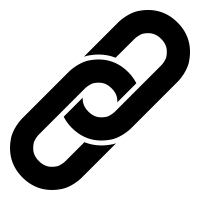
\includegraphics[height=8pt]{Screenshots/chainlink.png}: Indicates linked markers. Markers with the same number are linked and all of them move when one changes its position
\item \textbf{Trace:} The trace name the marker is assigned to
\item \textbf{Type:} Various marker types are available, see section~\ref{marker:types}
\item \textbf{Settings:} Allows for configuration of the marker based on marker type
\item \textbf{Restrict:} Forces the marker to a specific frequency range (or power/time range if the trace uses another domain)
\item \textbf{Data:} The trace data at the marker position which can be displayed in different formats
\end{itemize}

Various other settings are also available in the \textbf{context menu}. The context menu can be reached by right-clicking the marker, either in the marker dock or on the marker symbol in any graph.

\subsection{Creating and deleting markers}
There are three ways to create a marker:
\begin{itemize}
\item Right-click a trace on a graph and select "Add marker here"
\item Use the "Add marker" button in the marker dock
\item Use the "Add markers to all traces" button in the marker dock to create a marker for each trace. The created markers are linked by default (see section~\ref{marker:linking})
\end{itemize}
Markers can be deleted by:
\begin{itemize}
\item Selecting "delete" in the context menu
\item Selecting the marker in the marker dock and either pressing \keys{DEL} or using the "Delete marker" button
\end{itemize}
\subsection{Marker Types}
\label{marker:types}
Every marker is of a specific type. The type determines how the marker position is calculated and influences the available marker data formats. Some marker types also include helper markers for showing additional trace points. The marker type can be changed in the marker dock or in the context menu.
\subsubsection{Manual}
\screenshot{1.0}{MarkerManual.png}
This is the default marker type. It can be positioned at any position by the user and will never move on its own.
\subsubsection{Maximum}
\screenshot{1.0}{MarkerMaximum.png}
The marker snaps to the maximum amplitude of the assigned trace (within the limits of the "restrict" column).
\subsubsection{Minimum}
\screenshot{1.0}{MarkerMinimum.png}
The marker snaps to the minimum amplitude of the assigned trace (within the limits of the "restrict" column).
\subsubsection{Delta}
\screenshot{1.0}{MarkerDelta}
The delta marker can be positioned by the user. It will show the trace data relative to its assigned reference marker. The reference marker is selected by its marker number in the "type" column.
\subsubsection{Peak Table}
\screenshot{1.0}{MarkerPeakGraph.png}
\screenshot{1.0}{MarkerPeakTable.png}
The peak table lists all peaks in the signal above a specified signal level. It will create a helper marker for each peak. The peak threshold level can be adjusted in the "settings" column.
\subsubsection{Lowpass}
\screenshot{1.0}{MarkerLowpassGraph.png}
\screenshot{1.0}{MarkerLowpassTable.png}
The lowpass marker determines the cutoff frequency of a lowpass filter. At first the filter attenuation is calculated by finding the maximum signal amplitude. Afterward, the cutoff frequency is determined by finding the frequency at which the signal level has dropped by a specified amount. The threshold for this signal level drop can be adjusted in the "settings" column.

This marker type is only available for through measurements.
\subsubsection{Highpass}
\screenshot{1.0}{MarkerHighpassGraph.png}
\screenshot{1.0}{MarkerHighpassTable.png}
The highpass marker determines the cutoff frequency of a highpass filter. At first the filter attenuation is calculated by finding the maximum signal amplitude. Afterward, the cutoff frequency is determined by finding the frequency at which the signal level has dropped by a specified amount. The threshold for this signal level drop can be adjusted in the "settings" column.

This marker type is only available for through measurements.
\subsubsection{Bandpass}
\screenshot{1.0}{MarkerBandpassGraph.png}
\screenshot{1.0}{MarkerBandpassTable.png}
The bandpass marker determines the center frequency and bandwidth of a highpass filter. At first the filter attenuation is calculated by finding the maximum signal amplitude. Afterward, the cutoff frequency in each direction is determined by finding the frequency at which the signal level has dropped by a specified amount. The threshold for this signal level drop can be adjusted in the "settings" column. Finally, the center frequency is set to the middle of the higher and lower cutoff frequency.

This marker type is only available for through measurements.
\subsubsection{TOI/IP3}
\screenshot{1.0}{MarkerTOIGraph.png}
\screenshot{1.0}{MarkerTOITable.png}
This marker type calculates the third-order intercept point. It is only available in spectrum analyzer mode. Initially a peak search is executed to find the two highest peaks. Helper markers suffixed with "p", that show these peaks, are added to the parent marker. These helper markers show up on the graph and in the marker dock by clicking the expand/collapse arrow to the left of the marker \#. The frequencies of the intermodulation products are calculated from the two peak helper markers and a new helper marker is placed at each of these frequencies. One suffixed "l" to the left of the first peak and one suffixed "r" to the right of the second peak. Finally, the third-order intercept point as well as the tone and distortion signal amplitudes are calculated.
\subsubsection{Phase noise}
\screenshot{1.0}{MarkerPhasenoiseGraph.png}
\screenshot{1.0}{MarkerPhasenoiseTable.png}
This marker type calculates the phase noise of a signal. Is is only available in spectrum analyzer mode. Initially a peak search is executed to determine the signal frequency. Afterwards, a helper marker is placed at a specified offset. The offset can be configured in the "settings" column. By using the signal amplitudes from the peak and the offset marker, the phase noise is calculated.

\subsubsection{P1dB}
\screenshot{1.0}{MarkerP1dBGraph.png}
\screenshot{1.0}{MarkerP1dBTable.png}
This marker type is only available for through measurements on power sweeps. It calculates the 1dB compression point of amplifiers.

\subsection{Marker Data}
The trace data at the marker position can be displayed in the marker dock and on the graphs in various formats. The available formats depend on the marker type as well as the domain of the trace data. Only one of the available formats can be displayed in the marker dock at a time. On graphs, any amount of formats can be displayed at once. The shown formats can be selected in the context menu of the marker.

\begin{footnotesize}
\begin{center}
\begin{threeparttable}
\begin{tabularx}{\textwidth}{L{3cm}|X|L{7cm}}
    \toprule
    \textbf{Trace domain} & \textbf{Marker type} & \textbf{Available data formats}\\
     \hline
      \multirow{3}{*}{Time}  	&    \multirow{3}{*}{\makecell{Manual\\Delta}} & dB\\ 
    \cline{3-3}
        	&   & Real/Imaginary\\ 
    \cline{3-3}
        	&  & Impedance (if step response available) \\ 
    \cline{1-3}

      \multirow{5}{*}{\makecell{Time (zero span)\\ in SA mode}}  &    \multirow{5}{*}{\makecell{Manual\\Delta\\Maximum\\Minimum\\Peak Table}} & dBm\\ 
    \cline{3-3}
        	&   & dBuV\\ 
    \cline{3-3}
        	&  & Noise \\ 
	& & \\
	& & \\
    \cline{1-3}

      \multirow{9}{*}{\makecell{Time (zero span)\\ in VNA mode}}  &    \multirow{9}{*}{\makecell{Manual\\Delta\\Maximum\\Minimum\\Peak Table}} & dB\\ 
    \cline{3-3}
        	&   & dB + angle\\ 
    \cline{3-3}
        	&  & Real/Imaginary \\ 
    \cline{3-3}
	& & \multirow{6}{*}{$\left.\begin{array}{l}
$Impedance$\\
$VSWR$\\
$Series Resistance$\\
$Capacitance$\\
$Inductance$\\
$Quality factor$\\
                \end{array}\right\rbrace $\makecell{Only for reflection\\measurements}$$} \\
	& &  \\
	& & \\
	& &  \\
	& &  \\
	& &   \\
    \cline{1-3}

      \multirow{10}{*}{\makecell{Frequency\\ in SA mode}}  &    \multirow{5}{*}{\makecell{Manual\\Delta\\Maximum\\Minimum\\Peak Table}} & dBm\\ 
    \cline{3-3}
        	&   & dBuV\\ 
    \cline{3-3}
        	&  & Noise \\ 
	& & \\
	& & \\
    \cline{2-3}
	& \multirow{2}{*}{Phase Noise} & Phase Noise\\
   \cline{3-3}
	& & dB\\ 
    \cline{2-3}
	& \multirow{3}{*}{TOI/IP3} & third-order intercept\\
   \cline{3-3}
	& & Average tone level\\ 
   \cline{3-3}
	& & Average modulation product level\\ 
    \cline{1-3}


      \multirow{13}{*}{\makecell{Frequency\\ in VNA mode}}  &    \multirow{9}{*}{\makecell{Manual\\Delta\\Maximum\\Minimum\\Peak Table}} & dB\\ 
    \cline{3-3}
        	&   & dB + angle\\ 
    \cline{3-3}
        	&  & Real/Imaginary \\ 
    \cline{3-3}
        	&  & Group Delay \\ 
    \cline{3-3}
	& & \multirow{6}{*}{$\left.\begin{array}{l}
$Impedance$\\
$VSWR$\\
$Series Resistance$\\
$Capacitance$\\
$Inductance$\\
$Quality factor$\\
                \end{array}\right\rbrace $\makecell{Only for reflection\\measurements}$$} \\
	& &  \\
	& & \\
	& &  \\
	& &  \\
	& &   \\
    \cline{2-3}
  	& \multirow{2}{*}{Bandpass} & Center and bandwidth\\
   \cline{3-3}
	& & Insertion loss\\ 
    \cline{2-3}
  	& \multirow{2}{*}{\makecell{Lowpass\\Highpass}} & Cutoff frequency\\
   \cline{3-3}
	& & Insertion loss\\ 
    \cline{2-3}
   \cline{1-3}

      \multirow{10}{*}{\makecell{Power}}  &    \multirow{10}{*}{\makecell{Manual\\Delta\\Maximum\\Minimum\\P1dB}} & 1dB compression point (only for P1dB type)\\ 
    \cline{3-3}
        	&   & dB \\ 
    \cline{3-3}
        	&   & dB + angle\\ 
    \cline{3-3}
        	&  & Real/Imaginary \\ 
    \cline{3-3}
	& & \multirow{6}{*}{$\left.\begin{array}{l}
$Impedance$\\
$VSWR$\\
$Series Resistance$\\
$Capacitance$\\
$Inductance$\\
$Quality factor$\\
                \end{array}\right\rbrace $\makecell{Only for reflection\\measurements}$$} \\
	& &  \\
	& & \\
	& &  \\
	& &  \\
	& &   \\
    \hline

      \bottomrule
\end{tabularx}
\end{threeparttable}
\end{center}
\end{footnotesize}

\subsection{Linking markers}
\label{marker:linking}
Normally, markers can be moved individually and are only connected to one trace. This creates a problem when reading out trace data from multiple traces at the same position. If the position is changed, all markers need to be moved manually to the new position. Linked markers provide a solution to this problem: All markers within a linked group always use the same position. If one marker is moved, the others move as well. The linked group of each marker is indicated in the marker dock (empty if the marker does not belong to any linked group).

Only markers that are movable can be added to linked groups. Markers that perform automatic positioning (e.g. a marker with the type maximum) cannot be added to a linked group.

\subsubsection{Creating a new linked group}
Select multiple markers in the marker dock, right-click and select "link selected".
\subsubsection{Adding a marker to an existing linked group}
Open the marker's context menu, choose "Add to linked group" and select the linked group the marker should be added to.
\subsubsection{Removing a marker from a linked group}
\begin{itemize}
\item Open the marker's context menu, choose "Remove from linked group"
\item Select multiple linked markers in the marker dock, right-click and select "Break links" to remove all selected markers from their linked groups.
\end{itemize}

\section{Compound Device}
The LibreVNA supports combining multiple hardware units into a "Compound Device". When used, the configured physical LibreVNAs are combined into a virtual device with more ports. When connected to such a device, additional measurement paramaters are available (e.g. measuring S23 in VNA mode or port 3 in spectrum analyzer mode).

\begin{important}
When connected to a compound device and in VNA mode, there is no phase information for through measurements between different physical devices. This is a hardware limitation and the phase is set to zero in the software. Through measurements within a physical device and all reflection measurements retain their phase information.
\end{important}

\subsection{Creating a compound device}
Compound devices must be configured in the preferences:\linebreak\menu[,]{Window,Preferences,Device Drivers,LibreVNA/Compound}
\screenshot{1.0}{CompoundDeviceList.png}
Create and remove compound devices with the buttons on the right. Edit an existing compound device by double-clicking it:
\screenshot{1.0}{CompoundDeviceEdit.png}
Required steps when creating a compound device:
\begin{enumerate}
\item Assign a name to the new compound device
\item Select the synchronization method between devices. At the moment, only GUI synchronization is supported but future hardware versions might support faster synchronization via dedicated trigger ports
\item Drag-and-drop a LibreVNA symbol into the configuration area for every physical device in the compound device
\begin{itemize}
\item At least two physical devices must be used
\item At most four physical devices can be combined with a maximum of eight virtual ports
\end{itemize}
\item Assign serial numbers to each physical device. Serial numbers for all currently connected devices are available in the dropdown but it is also possible to enter a different serial number manually
\item Assign the virtual ports of the compound device:
\begin{itemize}
\item Each port number must appear only once
\item Port numbers must start with port 1
\item Port numbers must be consecutive, e.g. port 1,2 and 4 is not allowed because port 3 is missing
\item Physical ports may be left unused
\end{itemize}
\end{enumerate}

\subsection{Connecting to a compound device}
Configured compound devices appear in the device list when all required physical devices are connected. Once connected, new measurements or ports are available depending on the number of configured ports in the compound device.

\begin{information}
Through measurements between physical devices depend on precise matching of the stimulus frequency. Depending on the accuracy of the internal frequency source and the selected IF bandwidth, the stimulus signal from the generating device may fall outside of the IF bandwidth of the receiving device, resulting in a reported lower amplitude than actually present. Either align both internal oscillators precisely with the frequency calibration or (recommended) switch to using the external reference input when using a compound device.
\end{information}

\subsection{Limitations}
Certain features are not available when connected to a compound device. To use them, disconnect from the compound device and connect directly to the individual physical devices:
\begin{itemize}
\item Firmware update
\item Manual control
\item Source calibration
\item Receiver calibration
\item Frequency calibration
\end{itemize}


\section{Amplitude Calibration}
\label{amplitude:calibration}
This section is about calibrating the source output level and spectrum analyzer level. It does not affect VNA measurements at all. For the VNA calibration, see section~\ref{vna:calibration}.

Both the internal signal source and the receiver paths used in the signal generator or spectrum analyzer modes have no means of ensuring accurate amplitudes (as imperfections are removed by the VNA calibration, the hardware is not optimized for absolute amplitude accuracy). Frequency dependent amplitude calibrations are available in order to improve the accuracy of both the signal generator and the spectrum analyzer (especially when the tracking generator option is enabled in the spectrum analyzer). These calibrations are permanently stored in the device and are only required to be performed once. The \textbf{Source Calibration} corrects the output of the signal generator and the spectrum analyzer's tracking generator, while the \textbf{Receiver Calibration} corrects the measurement of the spectrum analyzer.

For both calibrations, other test equipment is required, ideally covering the whole range of \SI{1}{\mega\hertz} to \SI{6}{\giga\hertz} (a calibration of only the partial frequency range is also possible but signals/measurements outside the calibrated range will be inaccurate). The Source Calibration requires a way to measure the output of the \vna{} (e.g. a spectrum analyzer or power meter), the Receiver Calibration requires a signal source (e.g. a signal generator). Once either calibration has been completed, the \vna{} can also infer the other one with reasonable accuracy.

\subsection{Source Calibration}
Select \menu[,]{Device,Source Calibration}. A window showing the current source calibration opens:
\screenshot{1.0}{SourceCalibration.png}
These are the necessary steps:
\begin{enumerate}
\item \textbf{Set up the calibration frequencies:} Add or remove points according to your needs. Ideally, they should be evenly spaced across the calibration range, maybe with a slight emphasis on higher frequencies (signal levels generally vary more at higher frequencies). Additionally, it is advisable to set one point at \SI{25}{\mega\hertz} and another point just below it (at \SI{25}{\mega\hertz} a band is switched, resulting in an amplitude discontinuity). Up to 64 points can be used.
\item \textbf{Select the calibration mode:} Either calibrate both ports separately (best accuracy but more work) or assume that they are identical and use the measurement at one port for both.
\item \textbf{Perform the calibration:} For each frequency and port, select the corresponding cell in the table. The \vna{} will generate a signal at the selected frequency, on the selected port, at (what it thinks is) \SI{-20}{\dBm}. Use your external equipment to determine the actual output level and enter it into the selected cell.
\item \textbf{Save the calibration:} Once all measurements have been taken, the "Save to Device" button becomes available. There is no way to save intermediate results, you have to calibrate all frequencies you have chosen in step 1.
\end{enumerate}
If you've already done a Receiver Calibration, it's possible to infer the Source Calibration from it. Press \keys{Automatic measurement}, connect both ports of the \vna{} directly to each other and press \keys{Start Measurement}. This connection should be as ideal as possible (short, low loss cable) as every imperfection directly translates into calibration errors. During the automatic calibration, the \vna{} uses the already established frequency points from the Receiver Calibration and measures the output amplitude by itself to determine the coefficients of the Source Calibration.
\subsection{Receiver Calibration}
Select \menu[,]{Device,Receiver Calibration}. The Receiver Calibration works almost identically to the Source Calibration. The only difference is in step 3:
\begin{enumerate}
\setcounter{enumi}{2}
\item \textbf{Perform the calibration:} For each frequency and port, select the corresponding cell in the table and apply a signal with known level at the selected frequency and port. The signal level should be in the range of \SI{-40}{\dBm} to \SI{-10}{\dBm}. Higher signal levels might already compress in the receiver while lower levels unnecessarily increase calibration errors due to noise. The \vna{} tunes its receiver to the selected frequency and measures the applied signal's amplitude. Enter the actual amplitude into the selected cell while the signal is still being applied. The signal should be applied for a minimum of \SI{2}{\second} to ensure an accurate measurement.
\end{enumerate}
\section{Troubleshooting}
\label{troubleshooting}
If there was an error in the boot process, the "Booting" LED will blink an error code repeatedly:
\begin{center}
\begin{threeparttable}
\begin{tabularx}{\textwidth}{L{1cm}|X|L{7cm}}
    \toprule
    \textbf{Error Code} & \textbf{Meaning} & \textbf{Possible solution}\\
     \hline
      1   	&      Failed to detect FLASH memory  & Hardware failure, check soldering\\
    \hline
      2   	&      Invalid FLASH content  & Perform firmware update\\
    \hline
      3   	&      Failed to configure FPGA & Check FPGA bitstream generator settings\\
    \hline
      4   	&      Hardware initialization failed & Verify that FPGA bitstream and uC firmware are created from the same release\\
      \bottomrule
\end{tabularx}
\end{threeparttable}
\end{center}
\end{document}
